\documentclass{article}
\newcommand{\blind}{0}
% if you need to pass options to natbib, use, e.g.:
\PassOptionsToPackage{numbers, compress}{natbib}
% before loading neurips_2021

% ready for submission
\usepackage[preprint]{neurips_2021}

% to compile a preprint version, e.g., for submission to arXiv, add add the
% [preprint] option:
%     \usepackage[preprint]{neurips_2021}

% to compile a camera-ready version, add the [final] option, e.g.:
     %\usepackage[final]{neurips_2021}

% to avoid loading the natbib package, add option nonatbib:
%\usepackage[nonatbib]{neurips_2021}

\usepackage[utf8]{inputenc} % allow utf-8 input
\usepackage[T1]{fontenc}    % use 8-bit T1 fonts
\usepackage{hyperref}       % hyperlinks
\usepackage{url}            % simple URL typesetting
\usepackage{booktabs}       % professional-quality tables
\usepackage{amsfonts}       % blackboard math symbols
\usepackage{nicefrac}       % compact symbols for 1/2, etc.
\usepackage{microtype}      % microtypography
\usepackage{xcolor}         % colors
\usepackage{multirow}     

\usepackage{amsmath,amssymb,dsfont,color,bm,mathtools,enumitem}
\mathtoolsset{showonlyrefs}
\usepackage{amsthm}
\usepackage{subcaption}

\newtheorem{thm}{Theorem}
\newtheorem{lem}{Lemma}
\newtheorem{prop}{Proposition}
\newtheorem{pro}{Property}
\newtheorem{cor}{Corollary}

\usepackage{caption}

\DeclareCaptionFont{mysize}{\fontsize{9}{9.6}\selectfont}
\captionsetup{font=mysize}

\theoremstyle{definition}
\newtheorem{defn}{Definition}
\newtheorem{assumption}{Assumption}
\newtheorem{example}{Example}
\newtheorem{rmk}{Remark}

% If you use BibTeX in apalike style, activate the following line:
%\bibliographystyle{apalike}
\input macros.tex
\usepackage{mathrsfs}  
\def\caliB{\mathscr{B}}
\usepackage{float}

\setlength{\bibsep}{0.0pt}

\begin{document}

\if1\blind
{   \title{Smooth tensor estimation with 
unknown permutations}
\author{%
  Chanwoo Lee \\
  University of Wisconsin-Madison\\
  \texttt{chanwoo.lee@wisc.edu} \\
  % examples of more authors
   \And
   Miaoyan Wang \\
   University of Wisconsin-Madison \\
   \texttt{miaoyan.wang@wisc.edu} }

    \maketitle
} \fi

\if0\blind
{
 \date{}
  \title{Smooth tensor estimation with unknown permutations}
\author{}
\maketitle
} \fi

\vspace{-.3cm}
\begin{abstract}
 We consider the problem of structured tensor denoising in the presence of unknown permutations. Such data problems arise commonly in recommendation system, community detection, and multiway comparison applications. Here, we develop a general family of smooth tensors up to arbitrarily index permutations; the model incorporates the popular block models and graphon models. We show that a constrained least-squares estimate in the block-wise polynomial family achieves the minimax error bound. A phase transition phenomenon is revealed with respect to the smoothness threshold needed for optimal recovery. In particular, we find that a polynomial of degree of $(m-2)(m+1)/2$ is sufficient for accurate recovery of order-$m$ tensors, whereas higher smoothness exhibits no further benefits. Furthermore, we provide an efficient polynomial-time Borda count algorithm that provably achieves optimal rate under monotonicity assumptions. The efficacy of our procedure is demonstrated through both simulations and Chicago crime date applications. 
\end{abstract}


\section{Introduction}\label{sec:int}
\vspace{-.1cm}
Higher-order tensor datasets arise ubiquitously in modern data science applications.
Tensor structure provides effective representation of data that classical vector- and matrix-based methods fail to capture. 
One example is music recommendation system that records ratings of songs from users on different contexts \citep{baltrunas2011incarmusic}. This three-way tensor of user$\times$song$\times$context allows us to investigate interaction of users and songs under a context-specific manner.
Another example is network analysis that studies the connection pattern among nodes.  Pairwise interactions are often insufficient to capture the complex relationships, whereas multi-way interactions improve understanding the networks in social sciences \citep{gao2021minimax} and recommendation system \citep{han2020exact}. In both examples, higher-order tensors represent multi-way interactions in an efficient way.


%Tensor estimation problem cannot be solved without imposing structure. An appropriate reordering of tensor entries can provide effective representation of the hidden signal structure. For example, consider the  music recommendation system \citep{baltrunas2011incarmusic}. Suppose that we have a certain criterion available (such as similarities of music genres, age of users, and positive versus negative effect of  contexts) to reorder songs, users, and contexts with. Then, the sorted tensor has smooth structure because the entries from similar groups tend to have close values. Another example is hypergraph analysis. Hypergraph considers multi-way interactions of nodes and has hyperedges connecting more than two nodes. If we know the characteristics of individual nodes and rearrange them based on their similarities, the sorted adjacency tensor will have a special structure by the same reason.

\begin{figure}[h]
    \centering
    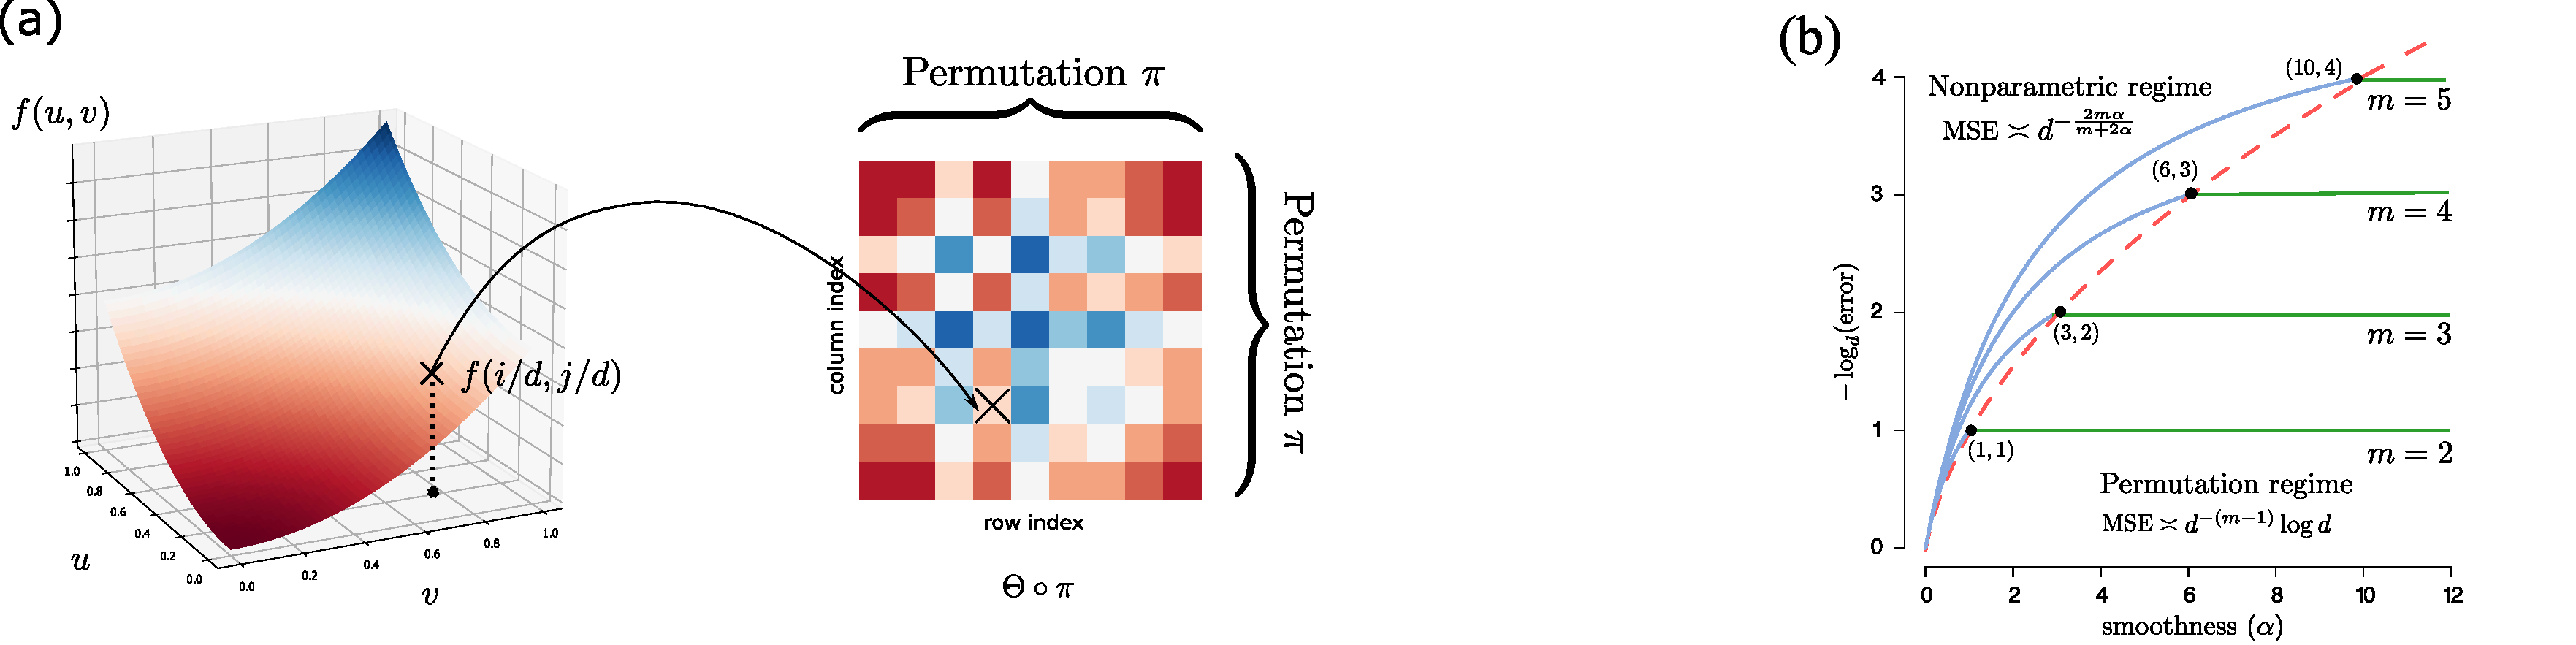
\includegraphics[width = .95\textwidth]{figures/semantic_new.pdf}
    \caption{(a): Illustration of order-$m$ $d$-dimensional permuted smooth tensor models with $m=2$. (b): Phase transition of mean squared error (MSE) (on -$\log d$ scale) as a function of smoothness
$\alpha$ and tensor order $m$. Bold dots correspond to the critical smoothness level above which higher
smoothness exhibits no further benefits to tensor estimation. See Theorems~\ref{thm:LSE}-\ref{thm:BC} in Sections~\ref{sec:lse}-\ref{sec:borda} for details.} \label{fig:rate}
   \vspace{-.2cm}
\end{figure}
Tensor estimation problem cannot be solved without imposing structure. We study a class of structured tensors, \emph{permuted smooth tensors}, of the following form:
\begin{equation}\label{eq:rep}
\tY=\Theta\circ \pi+\tE,\quad\text{where}\quad \Theta_{i_1,\ldots,i_m} = f\left({i_1\over d},\ldots,{i_m\over d}\right).
\end{equation}
where $\pi\colon[d]\rightarrow[d]$ is an \emph{unknown} latent permutation, $\Theta$ is an \emph{unknown} order-$m$ $d$-dimensional signal tensor, and $f$ is an \emph{unknown} multivariate function with certain notion of smoothness, $\Theta \circ \pi $ denotes the permuted tensor after reordering the indices along each of the $m$ modes, and $\tE$ is a symmetric noise tensor consisting of zero-mean, independent sub-Gaussian entries with variance bounded by $\sigma^2$. Figure~\ref{fig:rate}(a) shows an example of this generative model for the matrix case $m=2$. 
%where $\pi\colon[d]\rightarrow[d]$ is an unknown latent permutation,  $\Theta\in \mathbb{R}^{d\times \cdots\times d}$ is an unknown symmetric signal tensor, and $f$ is an unknown multivariate function with smoothness index $\alpha>0$ (see Figure~\ref{fig:rate}(a)), and $\tE$ is a symmetric noise tensor consisting of zero-mean, independent sub-Gaussian entries with variance bounded by $\sigma^2$. 
For ease of presentation, we focus on symmetric tensors; our models and techniques easily generalize to non-symmetric tensors.  Our primary goal is to estimate a permuted smooth signal tensor from a noisy observation~\eqref{eq:rep}.

{\bf Related work and our contributions.} The estimation problem of~\eqref{eq:rep} falls into the general category of structured learning with \emph{latent permutation}, which has recently observed a surge of interest. Models involving latent permutations include graphon~\cite{gao2021minimax,klopp2017oracle}, stochastic transitivity models~\cite{shah2019low}, and crowd labeling~\cite{li2019nearest}. Most of these methods are developed for matrices. The tensor counterparts are far less well understood. 


%We propose two estimating algorithms with accuracy guarantees: the least square estimation and Borda count estimation. 
The primary goal of our work is to provide statistical and computational estimation accuracy for the permuted smooth tensor model~\eqref{eq:rep}. Our major contributions are summarized below.
\vspace{-.2cm}
\begin{table*}[http]
    \centering
    \resizebox{\textwidth}{!}{%
    \begin{tabular}{c|cccc}
    & Pananjady et al~\cite{pananjady2020isotonic}&  Balasubramanian~\cite{balasubramanian2021nonparametric}&  Li et al~\cite{li2019nearest}&\textbf{Ours$^*$}\\
    \hline
       Model structure& monotonic & Lipschitz & Lipschitz &  $\alpha$-smoothness  \\
     Minimax lower bound& $\surd$  & $\times$ & $\times$ & $\surd$ \\
 Error rate for order-$m$ tensor$^*$ & \multirow{2}{*}{$d^{-1}$} & $d^{-{2m/(m+2)}}$ & $d^{-\lfloor m/3\rfloor }$ & $d^{-(m-1)}$ \\
       (e.g., when $m=3$) & & ($d^{-6/5}$) & $(d^{-1})$ & $(d^{-2})$ \\

     Polynomial algorithm& $\surd$ &$\times$ & $\surd$ & $\surd$\\
        \hline
    \end{tabular}
    }
    \caption{\small Comparison of our results with previous works. $^*$We  list here only the result for infinitely smooth order-3 tensors. Our results allow general tensors of arbitrary order $m$ and smoothness $\alpha$; See Theorems~\ref{thm:LSE}-\ref{thm:BC} in Sections~\ref{sec:lse}-\ref{sec:borda}.}\label{tab:comp}
\end{table*}
\vspace{-.3cm}
\begin{itemize}[wide,labelwidth=0pt, labelindent=0pt,itemsep=.4ex,topsep=-2pt]
\item We develop a general permuted $\alpha$-smooth tensor model, where $\alpha\geq 0$ is some natural measure of functional smoothness (formal definition in Section~\ref{sec:md}). In contrast to earlier work~\cite{balasubramanian2021nonparametric,li2019nearest}, we establish the statistically optima rate and fully characterize its dependence on tensor order, dimension, and smoothness index. Table~\ref{tab:comp} summarizes our improvement over previous works on tensor learning with latent permutations. 

%We establish the upper bound of the least-square estimate with high probability and show that this upper bound matches with minimax lower bound implying its optimality. 
\item We discover a phase transition phenomenon with respect to the smoothness threshold needed for optimal recovery in model~\eqref{eq:rep}. 
Figure~\ref{fig:rate}(b) plots the dependence of estimation error in terms of smoothness level $\alpha$ for tensors of order $m$. We find that the estimation accuracy improves with smoothness in the regime $\alpha \leq m(m-1)/2$, but then it becomes a constant of $\alpha$ in the regime $ \alpha > m(m-1)/2$. The phenomenon is distinctive from matrix problems~\citep{klopp2017oracle} and classical \emph{non-permuted} smooth function estimation, thereby highlighting the fundamental challenges in our new setting. 

\item We propose two estimation algorithms with accuracy guarantees: the least-squares estimation and Borda count estimation. The least-squares estimation is minimax optimal but computationally hard. The Borda count algorithm is polynomial-solvable, and we show it provably achieves the same optimal rate under extra monotonicity assumptions. Application to Chicago crime analysis is presented to showcase the usefulness of our method. The software package and all data used have been publicly released at CRAN.
\end{itemize}


{\bf Notation.} We use $[d]=\{1,\ldots,d\}$ for $d$-set with $d\in\mathbb{N}_{+}$. For a set $S$, $\mathds{1}_S$ denotes the indicator function. For positive two sequences $\{a_n\},\{b_n\}$,  we denote $a_n\lesssim b_n$ if $\lim_{n\to\infty} a_n/b_n\leq c$,  and $a_n\asymp b_n$ if $c_1\leq \lim_{n\to \infty} a_n/b_n\leq c_2$ for some constants $c,c_1,c_2>0$. Given number $a\in\mathbb{R}$, the floor function $\lfloor a\rfloor$ is the largest integer no greater than $a$, and the ceiling function $\lceil a\rceil$ is the smallest integer no less than $a$. An event $A$ is said to occur \emph{with high probability} if $\mathbb{P}(A)$ tends to 1 as the tensor dimension $d\to\infty$.We use $\Theta_{i_1,\ldots,i_m}$ to denote the tensor entry indexed by $(i_1,\ldots,i_m)$, and use $\Theta\circ\pi$ to denote the permuted tensor such that $(\Theta\circ\pi)_{i_1,\ldots,i_m} = \Theta_{\pi(i_1),\ldots,\pi(i_m)}$ for all $(i_1,\ldots,i_m)\in[d]^m$. We use $S(d)=\{\pi\colon [d]\to[d]\}$ to denote all possible permutations on $[d]$.


\section{Smooth tensor model with unknown permutation}\label{sec:md}
\vspace{-.1cm}
Suppose we observe an order-$m$ $d$-dimensional symmetric data tensor from the permuted tensors in \eqref{eq:rep}.
%Suppose we observe an order-$m$ $d$-dimensional data tensor from the following model,
%\begin{equation}\label{eq:obs}
%\tY=\Theta\circ \pi+\tE,
%\end{equation}
%where $\pi\colon[d]\rightarrow[d]$ is an unknown latent permutation,  $\Theta\in \bbR^{d\times \cdots \times d}$
%\begin{equation}\label{eq:rep}
%\tY=\Theta\circ \pi+\tE,\quad\text{where}\quad \Theta_{i_1,\ldots,i_m} = f\left({i_1\over d},\ldots,{i_m\over d}\right).
%\end{equation}
%where $\pi\colon[d]\rightarrow[d]$ is an unknown latent permutation,  $\Theta\in \mathbb{R}^{d\times \cdots\times d}$ is an unknown symmetric signal tensor represented by a multivariate function $f\colon[0,1]^m\rightarrow \mathbb{R}$, and $\tE$ is a symmetric noise tensor consisting of zero-mean, independent sub-Gaussian entries with variance bounded by $\sigma^2$. For simplicity of presentation, we focus on symmetric tensors in the main paper; our models and techniques easily generalize to non-symmetric tensors. 
We assume the generating function $f$ is in the $\alpha$-H\"older smooth family. 
\begin{defn}[$\alpha$-H\"older smooth]
A function $f\colon [0,1]^m\rightarrow \mathbb{R}$ is $\alpha$-H\"older smooth, denoted as $f\in\tH(\alpha)$, if there exists a polynomial $\text{Poly}_{\lfloor \alpha\rfloor}(\mx-\mx_0)$ of degree  $\lfloor \alpha\rfloor$, such that 
\begin{align}\label{eq:defn}
    |f(\mx) - \text{Poly}_{\lfloor \alpha\rfloor}(\mx-\mx_0)| \leq C\|\mx-\mx_0\|_\infty^\alpha, \text{ for all $\mx,\mx_0\in [0,1]^m$ and a constant $C>0.$}
\end{align}
\end{defn}

In addition to the function class $\tH(\alpha)$, we define the smooth tensor class based on discretization~\eqref{eq:rep}, 
\begin{equation}\label{eq:function}
{\small \tP(\alpha)= \left\{\Theta\in\mathbb{R}^{d\times \cdots \times d} \colon\Theta(\omega) = f\left({\omega \over d}\right) \text{ for all } \omega=(i_1,\ldots,i_m) \in[d]^m \text{ and } f\in\tH(\alpha)\right\}.}
\end{equation}

Combining~\eqref{eq:rep} and~\eqref{eq:defn} yields our proposed \emph{permuted smooth tensor model}. 
The unknown parameters are the smooth tensor $\Theta \in \tP(\alpha)$ and latent permutation $\pi \in S(d)$. The model is visualized in Figure~\ref{fig:rate}(a) for the case $m=2$ (matrices). 

We give two concrete examples to show the applicability of our permuted smooth tensor model. 

\begin{example}[Four-player game tensor] Consider a four-player board game. Suppose there are in total $d$ players, among which all combinations of four have played against each other. The game results are summarized as an order-4 (asymmetric) tensor, with entries encoding the winner of the games. Our model is then given by
\begin{align}
\mathbb{E}(\tY_{i_1,\ldots,i_4})&=\mathbb{P}(\text{user $i_1$ wins over $(i_2,i_3,i_4)$})
=f\left({\pi(i_1)\over d},\cdots, {\pi(i_4)\over d}\right).
\end{align}
We can interpret the permutation $\pi$ as the unknown ranking among $d$ players, and the function $f$ the unknown four-players interaction. Operationally, players with similar ranking would have similar performance encoded by the smoothness of $f$. 
\end{example}

\begin{example}[Co-authorship networks] Consider co-authorship networks. Suppose there are in total $d$ authors. We say there exists a hyperedge between nodes $(i_1,\ldots,i_m)$ if the authors $i_1,\ldots,i_m$ have co-authored at least one paper. The resulting hypergraph is represented as an order-$m$ (symmetric) adjacency tensor. Our model is then expressed as
\begin{align}
    \mathbb{E}(\tY_{i_1,\ldots,i_m})&=\mathbb{P}(\text{authors $i_1,\ldots,i_m$ co-authored})
=f\left({\pi(i_1)\over d},\cdots, {\pi(i_m)\over d}\right).
\end{align}
In this setting, we can interpret the permutation $\pi$ as the affinity measures of authors, and the function $f$ represents the $m$-way interaction among authors. Our nonparametric model learns the unknown function $f$ from data. 

%check examples from~\cite{ke2019community}. 
\end{example}



% \subsection{Connection to previous work}\label{sec:priorwork}
% The signal model~\eqref{eq:rep} has close relation to two different problems: multivariate nonparametric regression and hypergraphon estimation. 

% First,  one may view the problem as the classical nonparametric regression problem modeling the mean $(\Theta\circ\pi)_{i_1,\ldots,i_m}$ from  a regression function $f$ with covariates $({i_1}/d,\ldots,{i_m}/d)$. However, in our setting, we cannot observed the permutation $\pi$, which makes the problem  more difficult. Unlike the classical nonparametric regression, the function $f$ should be estimated only from  the observed noisy tensor $\{\tY_{i_1,\ldots,i_m}\}$ without information of the permutation. 
% In addition, this unobserved permutation setting incurs identifiability issue. We cannot estimate both the function $f$ (equivalently $\Theta$) and the permutation $\pi$. To overcome this identifiability issue, we use the following mean squared error for the permuted signal tensor $\Theta\circ\pi$ to measure the performance of the estimation,
% \begin{align}
%     \frac{1}{d^m}\sum_{(i_1,\ldots,i_m)\in[d]^m}\left((\hat\Theta\circ\hat\pi)_{i_1,\ldots,i_m}-(\Theta\circ\pi)_{i_1,\ldots,i_m}\right)^2.
% \end{align}
% Leveraging the underlying structure in \eqref{eq:rep} and smoothness of the function $f$ (formal definition is deferred to Section~\ref{subsec:bm}), we overcome these difficulties and successfully estimate the signal tensor without observing the permutation.

% In addition, the model~\eqref{eq:rep} is related to hypergraphons. 
% A  hypergraph is a generalization of a graph in which an edge (called hyperedge) can join any number of vertices.  $m$-uniform hypergraph is a hypergraph of which all hyperedges have size $m$. The structure of $m$-uniform hypergraph is naturally represented by a $m$-order tensor. So one can view the problem \eqref{eq:gmd} as estimating the probability tensor generating the observed hypergraph.
% The theory of hypergraph limits has studied and introduce hypergraphons  \citep{gowers2007hypergraph,zhao2015hypergraph} similar to graphons, limits of a sequence of graph \citep{lovasz2006limits,diaconis2007graph,lovasz2012large}.    Unlike the matrix case where graphon is represented as a bivariate function~\citep{lovasz2012large}, however, hypergraphons for $m$-uniform hypergraphs should be represented as a $(2^m-2)$-variate function \citep{zhao2015hypergraph}. Due to exponential number of variates, the general hypergraphon suffers from  high sample complexity. 
% To overcome this issue, simple $m$-variate hypergraphons have been introduced recently for efficient estimation while trading off the model flexibility \citep{balasubramanian2021nonparametric,lyu2021latent}.
%  Although our model can be viewed as a simple $m$-variate hypergraphon, our main interests lie on the general estimation of the smooth signal tensor from noisy observation including both binary- and continuous-valued entries.

%\vspace{-.4cm}
%\section{Block-wise tensor approximation }\label{sec:tba}
%\vspace{-.3cm}
Our general strategy for estimating the signal tensor in model~\eqref{eq:function} is based on the block-wise tensor approximation. We first introduce the tensor block model~\citep{han2020exact}. Then, we extend the idea to block-wise polynomial approximation.


{\bf Tensor block model.} The tensor block model~\citep{han2020exact} describes a checkerbroad pattern in the signal tensor. Specifically, suppose that there are $k$ clusters in the tensor dimension $d$, and the clusters are represented by a clustering function $z\colon [d]\rightarrow  [k]$. Then, the tensor block model assumes that signal tensor $\Theta\in\mathbb{R}^{d\times \cdots \times d}$ takes values from a mean tensor $\tS\in\mathbb{R}^{k\times\cdots\times k}$ according to the clustering function $z$:
\begin{align}\label{eq:block}
    \Theta_{i_1,\ldots,i_m} = \tS_{z(i_1),\ldots,z(i_m)}, \quad \text{ for all } (i_1,\ldots,i_m)\in[d]^m.
\end{align}
A tensor $\Theta$ satisfying~\eqref{eq:block} is called a block-$k$ tensor. 
%Tensor block model have shown great success in discoverying hidden group structure for many applications~\citep{han2020exact}.
%Despite its popularity and great applicability, the tensor block models cannot describe delicate structure of the signal tensor when the tensor dimension $d$ is very large. 
Classical tensor block models aim to explain data with a finite number of blocks; this approach is useful when the sample outsizes the parameters. Our nonparametric models~\eqref{eq:rep}, by contrast, use infinite number of parameters to allow growing model complexity as sample increases. 
Therefore, we shift the goal of tensor block model from discovering hidden group structure to approximating the generative process of the function $f$ in~\eqref{eq:rep}. In our setting, the number of blocks $k$ should be interpreted as a resolution parameter (i.e., a bandwidth) of the approximation similar to the notion of number of bins in histogram and polynomial regression. 



{\bf Block-wise polynomial approximation.} The tensor block model~\eqref{eq:block} can be viewed as a discrete version of piece-wise \emph{constant} function. This connection motivates us to use block-wise \emph{polynomial} tensors to approximate $\alpha$-H\"older functions.  For a given block number $k$, we use $z\colon[d]\rightarrow [k]$ to denote the canonical clustering function that partitions $[d]$ into $k$ clusters,  $z(i) = \lceil ki/d\rceil,  \text{ for all } i\in[d].$
The collection of inverse images $\{z^{-1}(j)\colon j\in[k]\}$ consists of  disjoint and equal-sized subsets in $[d]$, and we have $\cup_{j\in[k]}z^{-1}(j) = [d]$ by the construction. We denote $\tE_k$ as the $m$-way partition as a collection of $k^m$ disjoint, equal-sized blocks in $[d]^m$, such that 
\begin{align}\label{eq:blockind}
    \tE_k = \{z^{-1}(j_1)\times\cdots\times z^{-1}(j_m)\colon (j_1,\ldots,j_m)\in [k]^m\}.
\end{align}
We refer to $\Delta\in \tE_k$ as the \emph{canonical blocks}. We propose to approximate the signal $\Theta$ in~\eqref{eq:rep} by degree-$\ell$ polynomial tensor within each block $\Delta \in \tE_k$. Specifically, we use $\caliB(k,\ell)$ to denote the class of block-$k$, degree-$\ell$ polynomial tensors,
\begin{align}
    \caliB(k,\ell) = \bigg\{&\tB\in(\mathbb{R}^d)^{\otimes m}\colon \tB(\omega) = \sum_{\Delta\in\tE_k}\text{Poly}_{\ell,\Delta}(\omega)\mathds{1}\{\omega\in\Delta\}\text{ for all } \omega\in[d]^m\bigg\},
\end{align}
where $\text{Poly}_{\ell,\Delta}(\cdot)$ denotes a degree-$\ell$ polynomial function in $\mathbb{R}^m$. Notice that degree-0 polynomial block tensor reduces to the tensor block model \eqref{eq:block}. We generalize the tensor block model to degree-$\ell$ polynomial block tensor, in a way analogous to the generalization from $k$-bin histogram to $k$-piece-wise polynomial regression.

%Smoothness of the function $f$ in \eqref{eq:rep} turns out to play an important role in the block-wise polynomial approximation.  The following lemma implies that we can always find block-wise polynomial tensor close to the signal tensor generated from $\alpha$-H\"older smooth function $f$.
%\begin{lem}[Tensor block approximation]\label{lem:approx}
%Suppose  $\Theta\in\tP(\alpha)$. Then,
%for every block number $k\leq d$, and degree $\ell\in\{0\}\cup\mathcal{N}_+$, we have the approximation error
%\begin{align}
%   \inf_{\tB\in\caliB(k,\ell)} \frac{1}{d^m}\FnormSize{}{\Theta-\tB}^2\lesssim \frac{m^2}{k^{2\min(\alpha,\ell+1)}}.
%\end{align}
%\end{lem}



\section{Fundamental limits via least-squares estimation}\label{sec:lse}
We develop two estimation methods based on the block-wise polynomial approximation. We first introduce a minimax optimal but computationally inefficient least-squares estimator as a statistical benchmark. In Section~\ref{sec:borda}, we will present a polynomial-time solvable estimator with provably same optimal rate under monotonicity assumptions.

We propose the least-squares estimation for model~\eqref{eq:rep} by minimizing the Frobenius loss under block-$k$, degree-$\ell$ polynomial tensor family $\caliB(k,\ell)$, 
\begin{align}\label{eq:lseopt}
    (\hat\Theta^{\text{LSE}},\hat \pi^{\text{LSE}}) &= \argmin_{\Theta\in\caliB(k,\ell), \  \pi\in S(d)}\FnormSize{}{\tY-\Theta\circ\pi}.
\end{align}
The least-squares estimator $(\hat\Theta^{\text{LSE}},\hat\pi^{\text{LSE}})$ depends on two tuning parameters: the number of blocks $k$ and the polynomial degree $\ell$. The optimal choice $(k^*,\ell^*)$ is provided in our next theorem. 
\begin{thm}[Least-squares estimation error]\label{thm:LSE} 
Consider the order-$m$ ($m\geq 2$) permuted smooth tensor model~\eqref{eq:rep} with $\Theta\in\tP(\alpha)$.
Then, the estimator $\hat\Theta^{\textup{LSE}}\circ\hat\pi^{\textup{LSE}}$  in \eqref{eq:lseopt} satisfies with high probability 
\begin{align}\label{eq:rates}
   \frac{1}{d^m}&\FnormSize{}{\hat\Theta^{\textup{LSE}}\circ\hat\pi^{\textup{LSE}}-\Theta\circ \pi}^2\lesssim  \begin{cases}d^{-{2m\alpha\over m+2\alpha}} & \text{ when } \alpha < m(m-1)/2,\\{\log d\over d^{m-1}}&\text{ when } \alpha \geq m(m-1)/2,
   \end{cases}
\end{align}
under the optimal choice of $\ell^* = \min(\lfloor\alpha\rfloor,(m-2)(m+1)/2)$ and $k^* = \lceil d^{m\over m+2\min(\alpha,\ell^*+1)}\rceil$.
\end{thm}
Theorem~\ref{thm:LSE} establishes the upper bound for the mean squared error of the least-squares estimator~\eqref{eq:lseopt}. We discuss the asymptotic error rates as $d\rightarrow \infty$ while treating the tensor order $m$ and smoothness $\alpha$ fixed. 
The least-squares estimation error has two sources of error: the nonparametric error $d^{-{2m\alpha\over m+2\alpha}}$ and the clustering error $\log d/d^{m-1}$.  When the function $f$ is smooth enough, estimating the function $f$ becomes relatively easier compared to estimating the permutation $\pi$. This intuition coincides with the fact that the clustering error dominates the nonparametric error when  $\alpha\geq m(m-1)/2$. 


We now compare our results with existing work in the literature. %Theorem~\ref{thm:LSE} shows that the best rate is obtained with the choice of  $(\ell^*, k^*) = (0,\lceil d^{1\over\alpha\wedge1+1}\rceil)$ in the matrix case ($m =2$). 
In the matrix case ($m=2$), our block-wise constant approximation and convergence rate reduce to the results in~\cite{klopp2017oracle}. For higher order tensor case ($m\geq 3$), earlier work~\citep{balasubramanian2021nonparametric} suggests that constant block approximation ($\ell^*=0$) remains minimax optimal for tensors. 
Our Theorem~\ref{thm:LSE} disproves this conjecture, and we reveal a much faster rate $d^{-(m-1)}$ compared to the conjectured lower bound $d^{-2m/( m+2)}$~\citep{balasubramanian2021nonparametric}. For example, permuted $\alpha$-smooth tensors of order-3 require quadratic approximation $(\ell^*=2)$ with $k^*\asymp d^{1/3}$ blocks, for all $\alpha\geq 2$. The results show the clear difference from matrices and highlight the challenges with tensors. 

The next theorem shows that the critical polynomial degree $(m-2)(m+1)/2$ $=[m(m-1)/2-1]$ is not only sufficient but also necessary for accurate estimation of order-$m$ permuted smooth tensors. 

\begin{thm}[Minimax lower bound]\label{thm:minimax} For any given $\alpha\in(0,\infty)$, the estimation problem based on model~\eqref{eq:rep} obeys the minimax lower bound 
\begin{equation}\label{eq:minimax}
\inf_{(\hat \Theta,\hat \pi)}\sup_{\Theta\in \tP(\alpha), \pi\in S(d)} \mathbb{P}\left({1\over d^m}\FnormSize{}{\Theta\circ \pi-\hat \Theta\circ \hat \pi}^2 \gtrsim d^{-{2m\alpha\over m+2\alpha}}+d^{-(m-1)}\log d \right) \geq 0.8.
\end{equation}
\end{thm}
The above result demonstrates that the upper bound~\eqref{eq:rates} is minimax optimal. Theorem~\ref{thm:minimax} is obtained via information-theoretical analysis and thus applies to all estimators including, but not limited to, the least-squares estimator~\eqref{eq:lseopt} and Borda count estimator introduced in next section. 


% There are two ingredients in the rate of convergence, the nonparametric rate $ d^{-2m(\alpha\wedge 1)\over m+2(\alpha\wedge 1)}$ and the clustering rate $\log d/d^{m-1}$.
% Depending on constants tensor order $m$ and smoothness $\alpha$, the convergence rate in \eqref{eq:rateMSE} becomes 
% \begin{align}
%      d^{-2m(\alpha\wedge1)\over m+2(\alpha\wedge1)}+\frac{\log d}{d^{m-1}}\asymp \begin{cases} d^{-2\alpha\over 1+\alpha}& m = 2, \alpha\in(0,1),\\ \log d/d & m =2, \alpha = 1,\\ d^{-2m(\alpha\wedge 1)\over m+2(\alpha\wedge 1)} & m>2.\end{cases}
% \end{align}
% Notice that the nonparametric rate dominates the clustering rate when $m>2$. The intuitive  explanation for this phenomenon is that when tensor order $m$ increases, the nonparametric estimation becomes harder because the number of parameters increases exponentially due to the possible $m$-combinations from $k$ clusters. On the other hand, the difficulty of clustering problem are almost the same regardless of tensor order $m$. This is because the number of clusters $k$ and tensor dimension $d$ remain the same.

\section{An adaptive and computationally feasible procedure}\label{sec:borda}
At this point, we should note that the least-squares estimation in \eqref{eq:lseopt} is generally computationally hard. In this section, we propose an efficient polynomial-time \emph{Borda count} algorithm with provably same optimal rate under the $\beta$-monotonicity condition. We first introduce $\beta$-monotonicity condition.  
\begin{defn}[$\beta$-monotonicity]\label{eq:defn}
A function $f\colon[0,1]^m \rightarrow \mathbb{R}$ is called $\beta$-monotonic, denoted as $f\in\tM(\beta)$, if 
\begin{align}\label{eq:monotonic}
    \left({i-j\over d}\right)^{1/\beta}\leq g(i)-g(j)\ \ \text{for all $i>j\in[d]$,} \quad \text{ where } g(i): = \frac{1}{d^{m-1}}\sum_{(i_2,\ldots,i_m)\in[d]^m} f\left({i\over d},{i_2\over d},\ldots,{i_m\over d}\right).
\end{align}
\end{defn}\vspace{-.3cm}
Our $\beta$-monotonicity condition extends the strictly monotonic degree condition in the graphon literature~\citep{chan2014consistent}; the latter is a special case of our definition with $\beta=1, m=2$. Our $\beta$-monotonicity condition is also related to isotonic functions~\citep{han2019isotonic,pananjady2020isotonic} which assume the coordinate-wise monotonicity, i.e., $f(x_1,\ldots,x_d)\leq f(x_1',\ldots,x_d')$
when $x_i\leq x_i'$ for $i\in[d]$. 

%This $\beta$-monotonicity condition allows to estimate the permutation $\pi$  in polynomial-time. 

%Before presenting the theoretical guarantees, we provide the intuition here. The parameter $\beta$ measures the difficulty of the problem for estimating the permutation $\pi$. Consider the noisy observation $\tY$ in  \eqref{eq:gmd}.
%We define the scores function $\tau\colon [d]\rightarrow\mathbb{R}$ as
%\begin{align}\label{eq:score}
%    \tau(i) = \frac{1}{d^{m-1}}\sum_{(i_2,\ldots,i_m)\in[d]^m} \tY_{i,i_2,\ldots,i_m}.
%\end{align}
%Then, the permuted score function $\tau\circ\pi^{-1}$ is equivalent to the function $g$ in \eqref{eq:monotonic} for the noiseless case.
%Therefore, we can find an estimate $\hat\pi$ that makes the permuted score function $\tau\circ\hat\pi^{-1}$ monotonically increasing. Notice that the estimated permutation $\hat\pi$ could be different from the oracle permutation $\pi$ due to the noise. We find that the larger $\beta$ guarantees the sharper consistency of $\hat\pi$. The large $\beta$ implies the large gaps of $|g(i)-g(j)|$ for $i\neq j\in[d]$. Therefore, we obtain similar ordering of $\{\tau(i)\}_{i=1}^d$ before and after the addition of the noise. This intuition is well represented by the following lemma.
%\begin{lem}[Permutation error]\label{lem:permute}
%Let $\hat\pi$ be the permutation that makes the permuted score function $\tau\circ \hat\pi^{-1}$  monotonically increasing. Then, we have
%\begin{align}
%   \textup{Loss}(\pi,\hat\pi):= \frac{1}{d}\max_{i\in[d]}|\pi(i)-\hat\pi(i)|\lesssim \left(\sigma d^{-(m-1)/2}\sqrt{\log d}\right)^{\beta},
%\end{align}
%with high probability.
%\end{lem}


Now we introduce a Borda count estimator that consists of two stages: sorting and block-wise polynomial approximation. The simplified version of the algorithm is described in Algorithm 1 and Figure~\ref{fig:borda}. 
\begin{figure}[H]
    \centering
    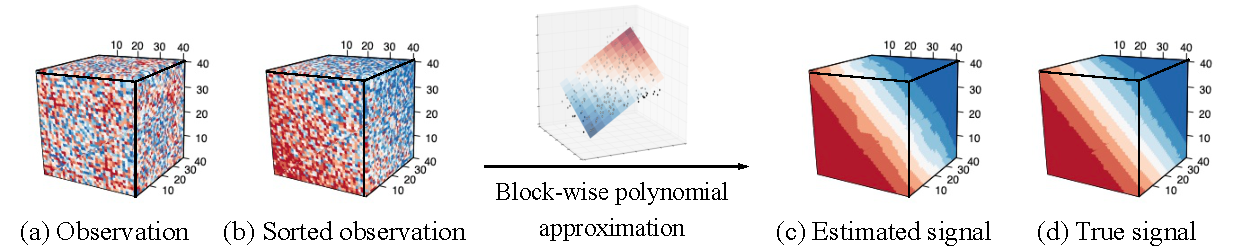
\includegraphics[width = .8\textwidth]{figures/Borda2.pdf}
    \caption{Procedure of Borda count estimation. We first sort the tensor entries using the proposed procedure. Then, we estimate the signal tensor using block-$k$ degree-$\ell$ polynomial approximation.}
    \label{fig:borda}
    \vspace{-.6 cm}
\end{figure}

\vspace{-.3cm}
\begin{center}
\includegraphics[width=1\textwidth]{figures/algorithm_template.pdf}
\end{center}
\vspace{-.4cm}
 %Notice that the least square estimation in \eqref{eq:lseopt} requires combinatoric search for the permutation resulting in exponential time complexity. However, optimization problem in Algorithm 1 only requires to estimate the degree-$\ell$ polynomial block tensor. Therefore, this step reduces to a degree-$\ell$ polynomial regression problem within each block $\tE_k$.  
%\vspace{-.2cm}
%\subsection{Computational and statistical complexity}
%\vspace{-.2cm}
%%\paragraph{Complexity of the algorithm.}
%The complexity of the Borda count algorithm can be computed separately in each stage.
%In the sorting stage, computing the score function $\tau$  requires $\tO(d^{m-1})$ additions while sorting the $\tau(1),\ldots,\tau(d)$ takes about $\tO(d\log d)$ comparisons. In block-wise polynomial approximation stage, we compute $k^m$ different  degree-$\ell$ polynomial tensors. For each  degree-$\ell$ polynomial tensor,  $\tO((d/k)^m\ell)$ arithmetic operations are needed. Thus, the second step requires $\tO(d^m\ell)$ arithmetic operations.  Combining these two steps yields the total complexity at most $\tO(d^m\log d)$.

%\paragraph{Consistency of Borda count estimation.}
\begin{thm}[Estimation error for Borda count; simplified version]\label{thm:BC}
Suppose that the signal tensor $\Theta$ is generated as in \eqref{eq:rep} with $f\in\tH(\alpha)\cap \tM(\beta).$
Then estimators $(\hat\Theta^{\text{BC}},\hat\pi^{\text{BC}})$ from Algorithm 1 satisfies
\begin{align}\label{eq:BC}
   \frac{1}{d^m}&\FnormSize{}{\hat\Theta^{\textup{BC}}\circ\hat\pi^{\textup{BC}}-\Theta\circ \pi}^2\lesssim 
    \begin{cases}d^{-{2m\alpha\over m+2\alpha}} & \text{ when } \alpha <c(\alpha,\beta,m),\\
    \left({\log d\over d^{m-1}}\right)^{\beta\min(\alpha,1)}&\text{ when } \alpha \geq c(\alpha,\beta,m),
    \end{cases}
\end{align}
with high probability under the optimal choice of $\ell^* = \min(\lfloor\alpha\rfloor,\lfloor c(\alpha,\beta,m)\rfloor)$ and $k^* = \lceil d^{m\over m+2\min(\alpha,\ell^*+1)}\rceil$.  Here $c(\alpha,\beta,m)>0$ is a constant only depending on $\alpha,\beta$,  and $m$.
\end{thm}
Theorem~\ref{thm:BC} shows the estimation consistency of Borda count estimator. We find that the Borda count estimator achieves the same minimax-optimal rate as the least-squares estimator under $1$-monotonicity condition. The least-squares estimator requires a combinatoric search with exponential-time complexity. By contrast, Algorithm 1 requires only the estimation of degree-$\ell$ polynomials within $k$ \emph{canonical blocks}. Therefore, the Borda count estimator is polynomial-time efficient. 



\section{Numerical experiments and data application}\label{sec:sim}
\vspace{-.1cm}
{\bf Numerical comparisons.} We simulate symmetric order-3 $d$-dimensional tensors based on the permuted smooth tensor model~\eqref{eq:rep} with function $f$ in Figure~\ref{fig:area}a. The detailed simulation procedure is described in Appendix. We assess the performance for the four popular tensor methods: (a) Spectral method ({\bf \small Spectral})~\citep{xu2018rates} on unfolded tensor; (b) Least-squares estimation ({\bf \small LSE})  with $\ell=0$ implied by~\citep{gao2021minimax}; (c) Lease square estimation ({\bf \small BAL}) implied by~\cite{balasubramanian2021nonparametric}; (d) Our {\bf \small Borda Count} algorithm. The performance accuracy is assessed via mean square error (MSE) $= d^{-3}\FnormSize{}{\Theta\circ\pi-\hat\Theta\circ\hat\pi}^2$. 

%Notice that considered functions cover a reasonable range of model complexities from low rank to high rank. We generate the entries of the noise tensor i.i.d. from Gaussian distribution $N(0,0.5^2)$. The permutation $\pi$ is randomly sampled from all permutations. 
%Throughout all experiments, we evaluate the accuracy of the estimation by mean square error (MSE) $= d^{-3}\FnormSize{}{\Theta\circ\pi-\hat\Theta\circ\hat\pi}^2$.

\vspace{-.3cm}
\begin{figure}[htp]
    \centering
    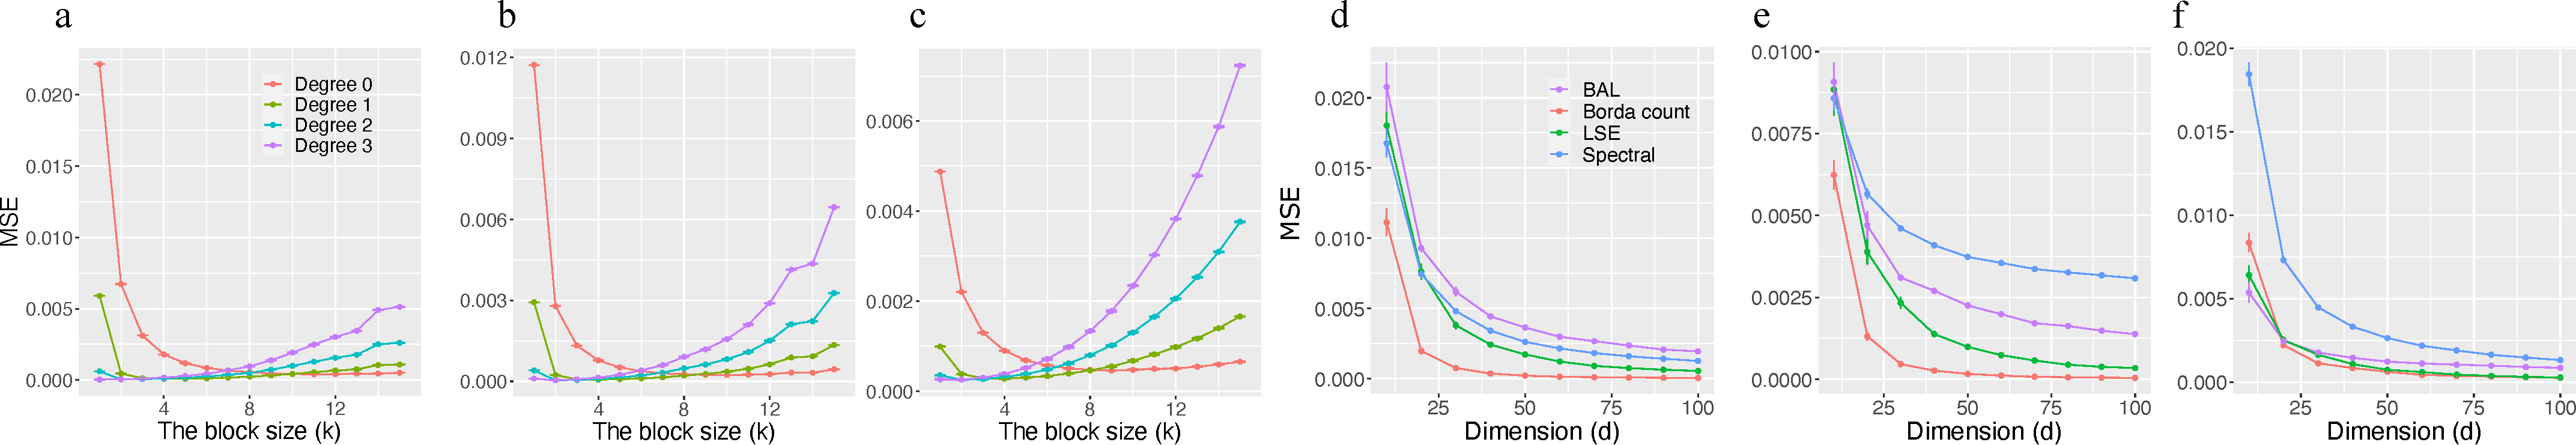
\includegraphics[width =\textwidth]{figures/sim2.pdf}    
    \caption{(a-c) MSE comparison versus the number of blocks under simulation models 1-3 respectively. (d-f) MSE comparison versus tensor dimension under models 1-3 respectively. MSEs are measured across $n_{\text{sim}} = 20$ replications.}
    \label{fig:degk}
    \vspace{-.3cm}
\end{figure}

Figure~\ref{fig:degk}a-c examines the impact of the block number $k$ and degree of polynomial $\ell$ for the approximation. We fix the tensor dimension $d = 100$, and vary the number of blocks $k\in\{1,\ldots,15\}$ and polynomial degree $\ell\in\{0,1,2,3\}.$ The result demonstrates the trade-off in accuracy determined by the number of blocks for each polynomial degree. We find that degree-2 polynomials give the smallest MSE among all considered approximation for order-3 tensors. These observations are consistent with our theoretical results in Sections~\ref{sec:lse}-\ref{sec:borda}. Figure~\ref{fig:degk}d-f shows that our algorithm {\bf \small Borda Count} achieves the best performance in all scenarios as the tensor dimension increases. The poor performance of {\bf \small Spectral} can be explained by the loss of multilinear structure in the tensor unfolding procedure. The sub-optimality of {\bf \small LSE} is possibly due to its limits in both statistics and computations. Statistically, our theorems have shown that constant block approximation has sub-optimal rates. Computationally, the least-squares estimation~\eqref{eq:lseopt} is highly non-convex and computationally unstable. The outperformance of {\bf \small Borda count} demonstrates the efficacy of our method.

\begin{figure}[h]
    \centering
    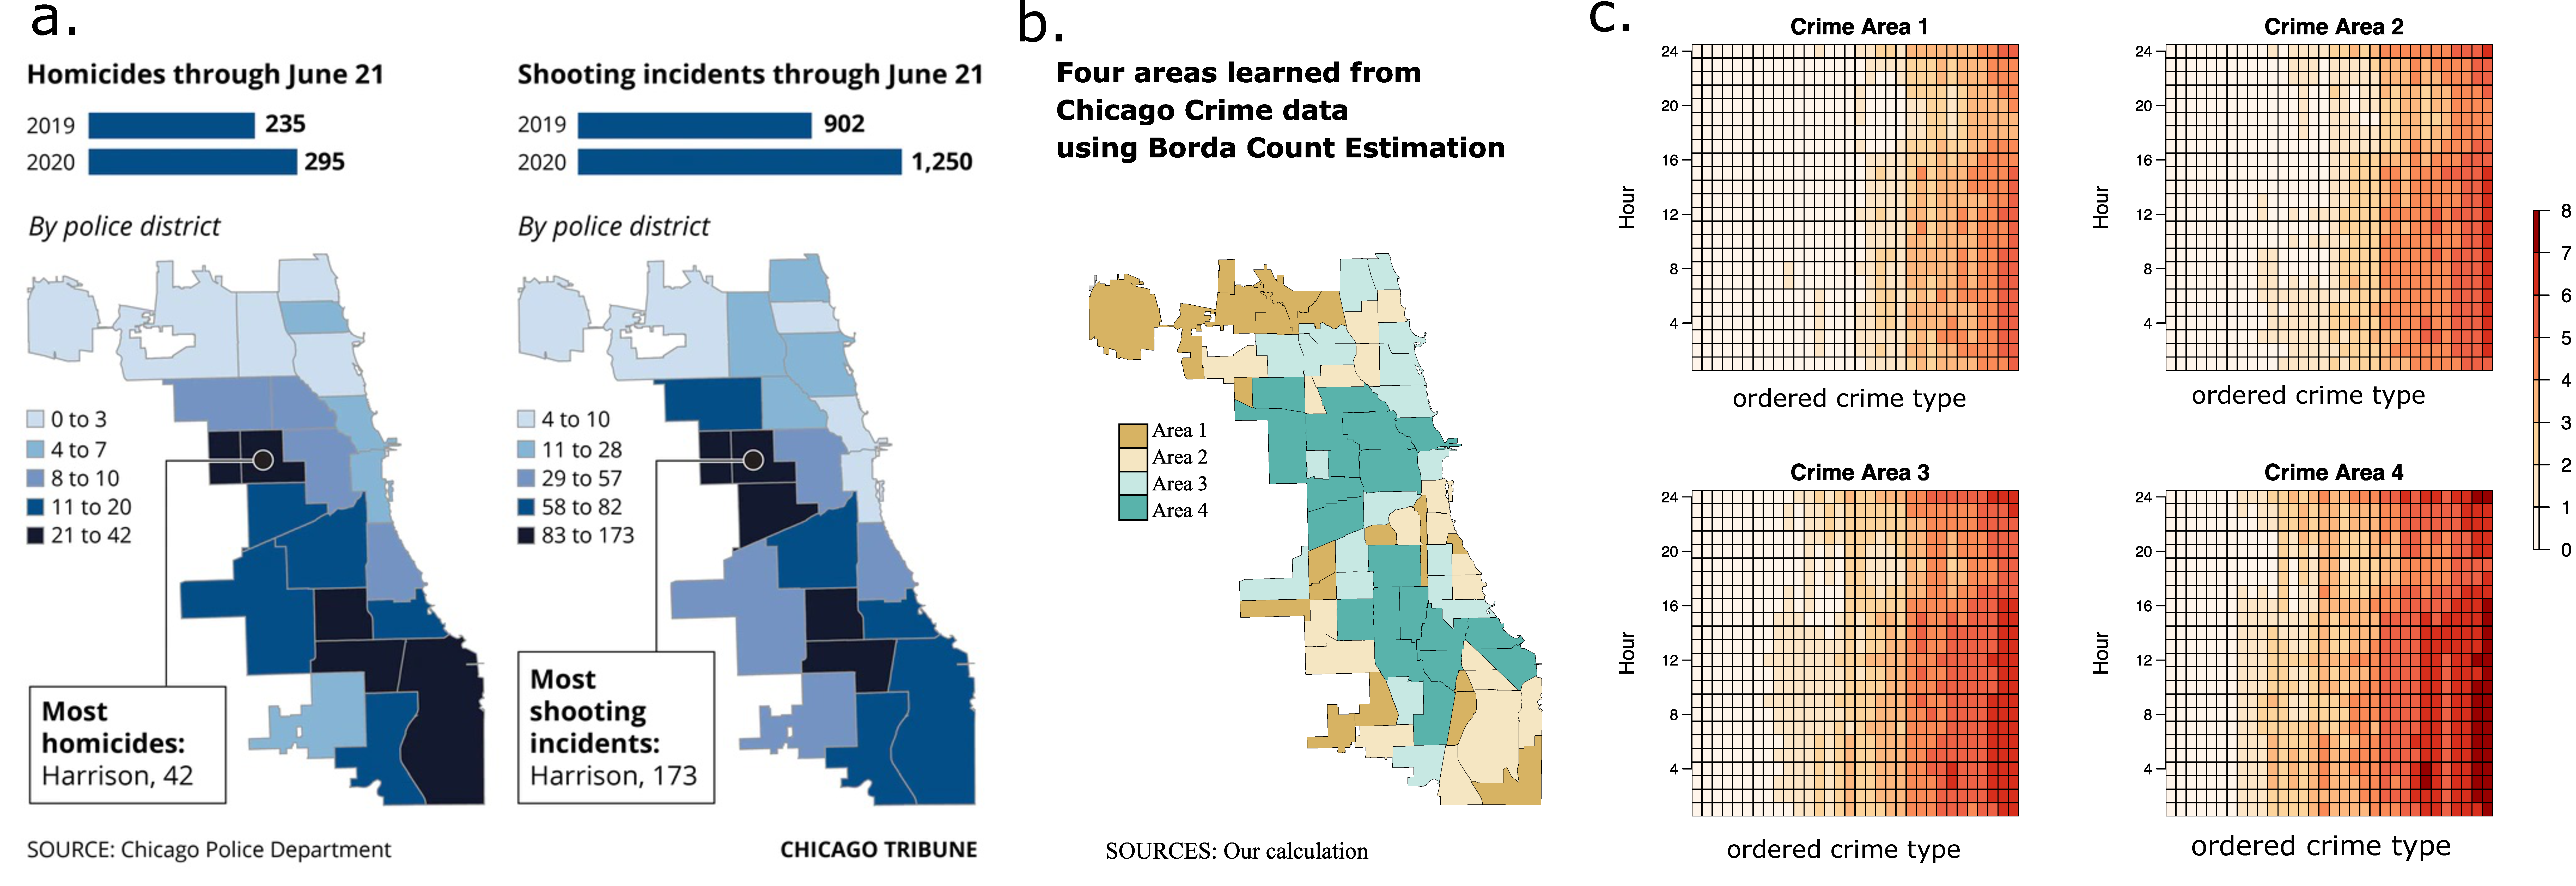
\includegraphics[width =1 \textwidth]{figures/drawing2.pdf}
    \caption{Chicago crime maps based on (a) \textit{Chicago Tribune} article in 2020 \citep{Jeremy.2020} and (b) our estimation using Borda Count algorithm. (c) Averaged log counts of crimes according to crime types, hours, and the four areas estimated by our Borda count algorithm. For space consideration, the annotated crime types are described in the Appendix.}
    \label{fig:area}
    \vspace{-.6cm}
\end{figure}

{\bf Applications to Chicago crime data.} Chicago crime tensor dataset is an order-3 tensor with entries representing the log counts of crimes from 24 hours, 77 Chicago community areas, and 32 crime types ranging from January 1st, 2001 to December 11th, 2017. We apply our Borda Count method to Chicago crime dataset. Cross validation result suggests the $(k_1,k_2,k_3)=(6,4,10)$, representing the block number for crime hours, community areas, and crime types, respectively.
We investigate the four clustered community areas obtained from our Borda Count algorithm. Figure~\ref{fig:area}a-b shows the four areas overlaid on a map of Chicago. We find that our clusters conform the actual locations even though our algorithm did not take any geographic information such as longitude or latitude. In addition, our clusters (Figure~\ref{fig:area}b) share similar geographical patterns with benchmark result (Figure~\ref{fig:area}a) based on \textit{Chicago Tribune} article in 2020 \citep{Jeremy.2020}. 
Figure~\ref{fig:area}c reveals that the major difference among four areas is the crime rates: Area 4 has the highest crime rates, and the crime rates monotonically decrease from Area 4 to Area 1. The variation in crime rates across hour and type, nevertheless, exhibits similarity among the four areas. For example, the number of crimes increases hourly from 8 p.m., peaks at night hours, and then drops to the lowest at 6 p.m. The interpretable similarities and differences among the four community areas demonstrate the applicability of our method in real data.


% \fixme{Miaoyan}{change ``Source; authors' calculation'' ``Sources: our calculation''.}


%Then, we examine the denoised signal tensor obtained from our method and analyze the trends between crime types and crime hours by the four community areas in Figure~\ref{fig:area}(b). Figure~\ref{fig:crimeA} shows the averaged log counts of crimes according to crime types and crime hours by four areas. We find that the major difference among four areas is the crime rates. Area 4 has the highest crime rates,  and the crime rates monotonically decrease from Area 4 to Area 1. The variation in crime rates across hour and type, nevertheless, exhibits similarity among the four areas. For example, Figure~\ref{fig:crimeA} shows that the number of crimes increases hourly from 8 p.m., peaks at night hours, and then drops to the lowest at 6 p.m. 
%The identified similarities and differences among the four community areas highlight the interpretability of our method in real data.
%\begin{figure}[h]
%    \centering
%    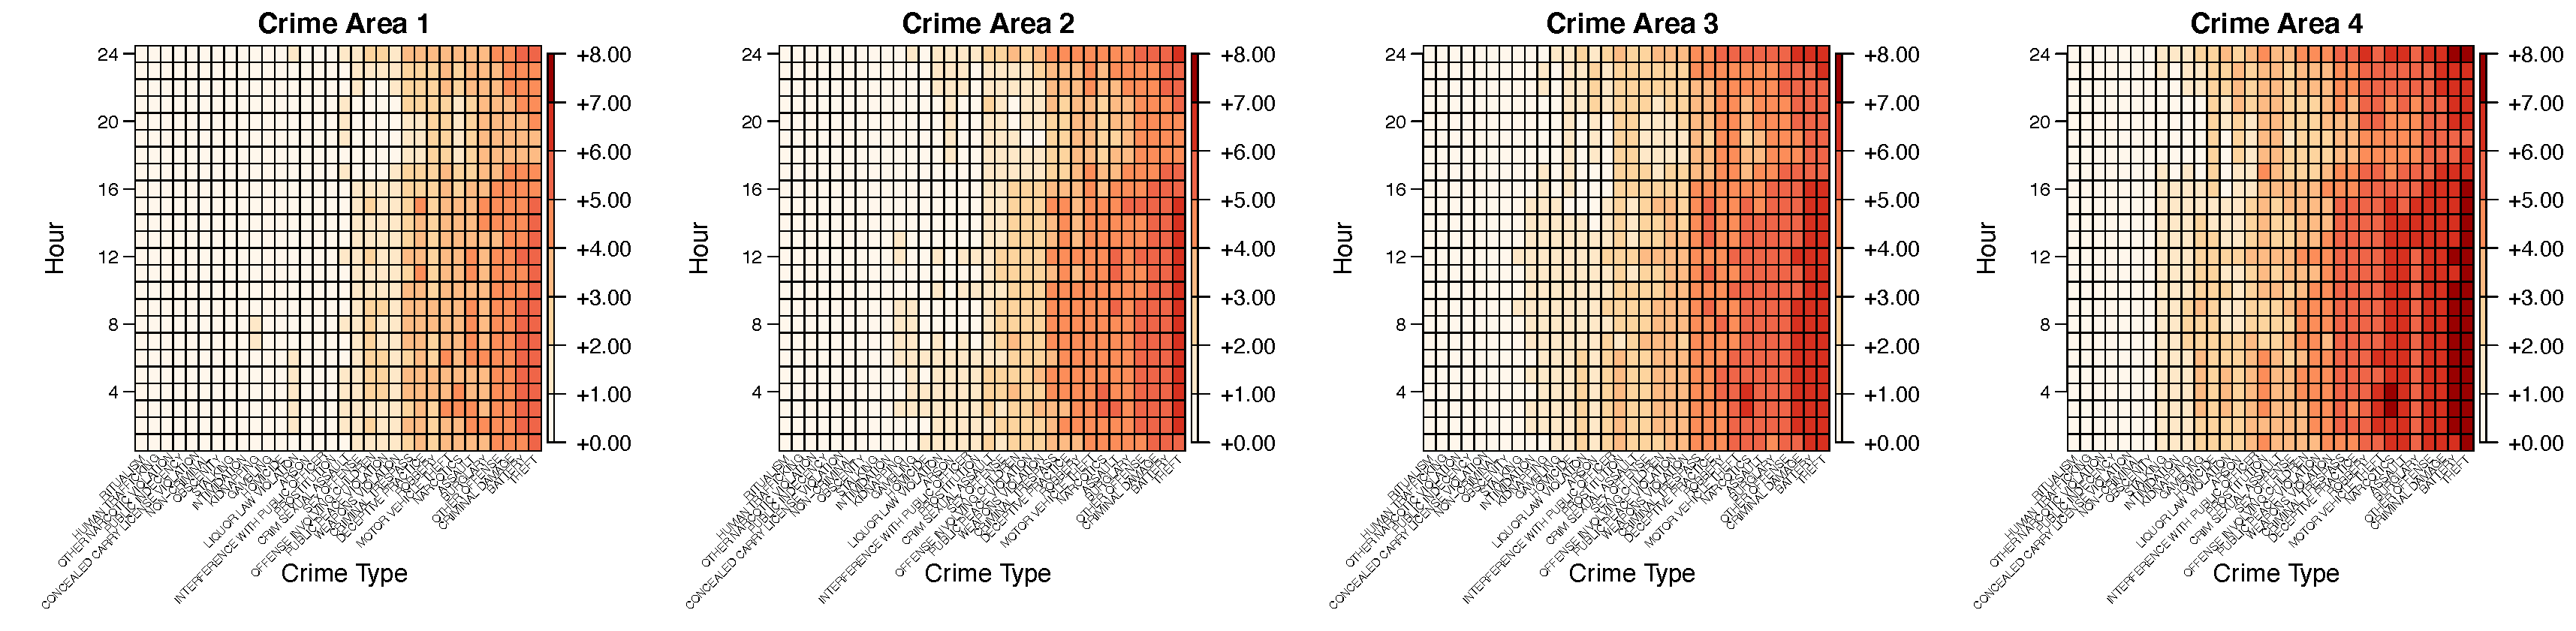
\includegraphics[width = \textwidth]{figures/CrimeAn.pdf}
%    \caption{Averaged log counts of crimes according to crime types, hours, and the four areas estimated by our Borda Count algorithm. We plot the estimated signal tensor entries averaged within four areas in the heatmap.}
%    \label{fig:crimeA}
%    \vspace{-.4cm}
%\end{figure}

\section{Conclusion}\label{sec:con}
We have presented a suite of statistical theory, estimation methods, and data applications for permuted smooth tensor models.
%An optimal error bound for the least square estimation is established based on block-wise polynomial approximation. Borda count estimation with polynomial algorithm is provided with the same convergence rate under $\beta$-monotonicity. 
We believe our results will be of interest to a very broad readership – from those interested in foundations of tensor methods to those in tensor data applications.  Our method will help the practitioners efficiently analyze tensor datasets in various areas. Toward this end, the software package and all data used have been publicly released at CRAN.
%The efficacy of our method is demonstrated through simulations and Chicago crime date analysis. Our method will help the practitioners efficiently analyze tensor datasets in various areas. Toward this end, the software package and all data used have been publicly released at CRAN.



% Acknowledgements should go at the end, before appendices and references

%\acks{We would like to acknowledge support for this project from the National Science Foundation (NSF grant IIS-9988642) and the Multidisciplinary Research Program of the Department of Defense (MURI N00014-00-1-0637). }

% Manual newpage inserted to improve layout of sample file - not
% needed in general before appendices/bibliography.



% Note: in this sample, the section number is hard-coded in. Following
% proper LaTeX conventions, it should properly be coded as a reference:

%In this appendix we prove the following theorem from
%Section~\ref{sec:textree-generalization}:                                                                                                                                                                                                                                                                                                                                                                                                                                                                                                                                                                                                                                                                                                                                                                                                                                                                                                                                                                                                                                            

{\small
\bibliographystyle{plain}
\bibliography{tensor_wang}
}
%%%%%%%%%%%%%%%%%%%%%%%%%%%%%%%%%%%%%%%%%%%%%%%%%%%%%%%%%%%%
% \section*{Checklist}

% %%% BEGIN INSTRUCTIONS %%%
% The checklist follows the references.  Please
% read the checklist guidelines carefully for information on how to answer these
% questions.  For each question, change the default \answerTODO{} to \answerYes{},
% \answerNo{}, or \answerNA{}.  You are strongly encouraged to include a {\bf
% justification to your answer}, either by referencing the appropriate section of
% your paper or providing a brief inline description.  For example:
% \begin{itemize}
%   \item Did you include the license to the code and datasets? \answerYes{}
%   \item Did you include the license to the code and datasets? \answerNo{The code and the data are proprietary.}
%   \item Did you include the license to the code and datasets? \answerNA{}
% \end{itemize}
% Please do not modify the questions and only use the provided macros for your
% answers.  Note that the Checklist section does not count towards the page
% limit.  In your paper, please delete this instructions block and only keep the
% Checklist section heading above along with the questions/answers below.
% %%% END INSTRUCTIONS %%%

% \begin{enumerate}

% \item For all authors...
% \begin{enumerate}
%   \item Do the main claims made in the abstract and introduction accurately reflect the paper's contributions and scope?
%     \answerYes{} See Section~\ref{sec:int}, {\bf Contributions.}
%   \item Did you describe the limitations of your work?
%     \answerYes{} We provide the limitation of the least square estimation in  Section~\ref{sec:borda}
%   \item Did you discuss any potential negative societal impacts of your work?
%     \answerNA{} This work does not present any foreseeble societal consequence
%   \item Have you read the ethics review guidelines and ensured that your paper conforms to them?
%     \answerYes{}
% \end{enumerate}

% \item If you are including theoretical results...
% \begin{enumerate}
%   \item Did you state the full set of assumptions of all theoretical results?
%     \answerYes{} The assumptions for main Theorems are fully state.
% 	\item Did you include complete proofs of all theoretical results?
%     \answerNo{}
% \end{enumerate}

% \item If you ran experiments...
% \begin{enumerate}
%   \item Did you include the code, data, and instructions needed to reproduce the main experimental results (either in the supplemental material or as a URL)?
%     \answerNo{}
%   \item Did you specify all the training details (e.g., data splits, hyperparameters, how they were chosen)?
%     \answerYes{} Training procedures are described in Section~\ref{sec:sim}
% 	\item Did you report error bars (e.g., with respect to the random seed after running experiments multiple times)?
%     \answerYes{} Error bars are provided in all Figures
% 	\item Did you include the total amount of compute and the type of resources used (e.g., type of GPUs, internal cluster, or cloud provider)?
%     \answerNo{}
% \end{enumerate}

% \item If you are using existing assets (e.g., code, data, models) or curating/releasing new assets...
% \begin{enumerate}
%   \item If your work uses existing assets, did you cite the creators?
%     \answerYes{} Data source has been cited in Section~\ref{sec:app}
%   \item Did you mention the license of the assets?
%     \answerNA{} No license available for teh assets used in this work.
%   \item Did you include any new assets either in the supplemental material or as a URL?
%     \answerTODO{}
%   \item Did you discuss whether and how consent was obtained from people whose data you're using/curating?
%     \answerNA{} The datasets are publicly available.
%   \item Did you discuss whether the data you are using/curating contains personally identifiable information or offensive content?
%     \answerNA{} No personally identifiable information is included in the datsets.
% \end{enumerate}

% \item If you used crowdsourcing or conducted research with human subjects...
% \begin{enumerate}
%   \item Did you include the full text of instructions given to participants and screenshots, if applicable?
%     \answerNA{} This work does not involve human subjects.
%   \item Did you describe any potential participant risks, with links to Institutional Review Board (IRB) approvals, if applicable?
%     \answerNA{} This work does not involve potential participant risk
%   \item Did you include the estimated hourly wage paid to participants. and the total amount spent on participant compensation?
%     \answerNA{} This work does not involve participants.
% \end{enumerate}

% \end{enumerate}

%%%%%%%%%%%%%%%%%%%%%%%%%%%%%%%%%%%%%%%%%%%%%%%%%%%%%%%%%%%%


\end{document}